\documentclass[12pt,a4paper]{article}
\usepackage[a4paper,top=4cm,left=4cm,right=3cm,bottom=3cm]{geometry}
\usepackage{amsmath,amssymb}
\usepackage{graphicx}
\usepackage{setspace}
\usepackage{enumitem}
\usepackage{fancyhdr}
\usepackage{lastpage}
\usepackage{microtype}
\sloppy
\onehalfspacing
\setlength{\parindent}{0pt}
\setlength{\parskip}{6pt}
\pagestyle{fancy}\fancyhf{}
\cfoot{Page \thepage\ of \pageref{LastPage}}
\renewcommand{\headrulewidth}{0pt}

\newcounter{para}
\newcommand{\p}{\refstepcounter{para}\textbf{[\thepara]}\ }

\begin{document}

\begin{center}
\textbf{FORM 2}\\[4pt]
\textbf{THE PATENTS ACT, 1970}\\
(39 of 1970)\\
\textbf{\&}\\
\textbf{THE PATENTS RULES, 2003}\\[10pt]
\textbf{PROVISIONAL SPECIFICATION}\\
(See section 10 and rule 13)
\end{center}

\vspace{6pt}
\textbf{1. TITLE OF THE INVENTION}

SYSTEM AND METHOD FOR SELECTIVE CHAOS CONTROL OF AUTONOMOUS AGENTS USING DIMENSION-WISE DIVERGENCE MEASUREMENT AND MINIMAL INTERVENTION

\textbf{2. APPLICANT}

\begin{tabular}{@{}lp{9cm}}
(a) Name: & KUHAN K\\
(b) Nationality: & Indian\\
(c) Address: & No.~1, Bharathidasan Nagar, Karaikal -- 609605, Puducherry, India
\end{tabular}

\textbf{3. PREAMBLE TO THE DESCRIPTION}

\textbf{PROVISIONAL}

The following specification describes the invention.

%% ==================================================================
\section*{FIELD OF THE INVENTION}

\p The present invention relates to the control of autonomous decision-making systems. More particularly, it relates to a system and method that measures, separately for each of a plurality of output dimensions, how strongly a small perturbation of the input is amplified in the output of an autonomous agent; that applies a corrective intervention only to those dimensions in which the amplification exceeds a threshold; that preserves controlled variability in dimensions designated as exploratory; and that schedules re-validation of multi-step agents according to an estimated error-growth rate. The autonomous agent may be a software agent driven by a generative model, a language-model-based database query generator, a planner of an autonomous robot or vehicle, or a monitoring system for physiological, behavioural or aggregate social time series.

%% ==================================================================
\section*{BACKGROUND OF THE INVENTION}

\p Autonomous agents built on large generative models produce an output by iterating a nonlinear map: each generated element is fed back as input for the next one, and in multi-step operation the results of earlier steps and of external tools are appended to the input. Such agents exhibit sensitive dependence on initial conditions. A small, meaning-preserving change in the input, such as a reworded instruction, a reordered list or a formatting change, or a single erroneous element early in the output, can lead to a substantially different final output. In multi-step operation such deviations grow and compound, so that the probability of completing a long task correctly falls sharply with task length.

\p In the theory of nonlinear dynamical systems, the rate at which nearby trajectories separate is quantified by the Lyapunov exponent, and an initial error $e_0$ grows to a tolerance $\Delta$ after a predictability horizon $T_h=\lambda^{-1}\ln(\Delta/e_0)$. Further, it is known from chaos-control methods (for example the Ott--Grebogi--Yorke method) that a chaotic system can be stabilised by small perturbations applied only when its trajectory leaves a target region.

\p Existing techniques for improving the reliability of generative agents have several limitations:
\begin{enumerate}[label=(\alph*)]
\item Uncertainty-estimation techniques, such as entropy over sampled answers or self-consistency checks, compute a single scalar score for the whole output. They do not identify which part of a structured output is unreliable.
\item Majority voting over complete outputs requires entire outputs to coincide. The probability that a sample is fully correct is the product of the per-part correctness probabilities and falls rapidly as the number of parts grows.
\item Verification of every step or every part of an output, and uniformly low sampling temperatures, suppress all variability equally. This increases computational cost (the number of model invocations), and it removes useful variability from parts of the output where diversity is desirable, such as alternative plans, explanations, or exploratory behaviour of a robot.
\item Re-validation of multi-step agents is performed at fixed intervals that do not adapt to how quickly a particular task diverges. Fast-diverging tasks are checked too rarely and slow ones too often.
\item In autonomous robots, exploratory or creative behaviour and safety constraints are typically handled by a single global setting, so that increasing exploration also increases the risk of unsafe actions.
\end{enumerate}

\p There is therefore a need for a system that localises instability to specific output dimensions, intervenes minimally and only where instability is harmful, deliberately retains controlled variability where it is beneficial, and schedules re-validation according to measured error growth.

%% ==================================================================
\section*{OBJECTS OF THE INVENTION}

\p The principal object of the invention is to provide a system and method for selective chaos control of an autonomous agent, in which instability is measured and controlled separately for each of a plurality of output dimensions.

\p Another object is to provide a dimension-wise divergence measure and a dimension-wise finite-step exponent computed from an ensemble of perturbed inputs. Together these form a ``chaos map'' of an output.

\p Another object is to estimate, without labelled data, an error-rate range for each output dimension from its observed divergence.

\p Another object is to provide a minimal-intervention controller for each dimension that selects the lowest-cost corrective action from an ordered intervention ladder only when the divergence of that dimension leaves a target band, thereby reducing the number of model invocations compared with verifying all dimensions.

\p Another object is to provide per-dimension variability control (``selective chaos''), in which precision dimensions are driven to low divergence while exploratory dimensions are held within a divergence band. The controller gain is limited below a computed critical value to prevent oscillation of the controller.

\p Another object is to provide an ``agent Lyapunov time'' and a predictability-horizon-based scheduler that triggers re-validation of a multi-step agent before its deviation reaches a tolerance.

\p A further object is to apply the above to autonomous robots, so that creative or exploratory decision dimensions remain varied while safety dimensions are held stable and unsafe actions are vetoed or corrected before actuation.

%% ==================================================================
\section*{SUMMARY OF THE INVENTION}

\p According to one aspect, the invention provides a system comprising at least one processor and a memory, the processor being configured to:
\begin{enumerate}[label=(\roman*)]
\item receive an input describing a task or situation;
\item generate a plurality $K$ of perturbed versions of the input, each preserving the meaning of the input, and determine a perturbation magnitude $\varepsilon$;
\item obtain from an agent a candidate output for each perturbed input;
\item decompose each candidate output into $D$ output dimensions by a decomposition module, each dimension being associated with a distance measure and with a role selected from at least a precision role and an exploratory (creative) role;
\item compute, for each dimension $j$, a divergence $d_j$ as the mean pairwise distance between the candidate values of that dimension, and a finite-step exponent $\lambda_j=\ln(\max(d_j,d_{\min})/\varepsilon)$;
\item for each precision dimension whose divergence lies within its target band, accept a consensus value of that dimension;
\item for each precision dimension whose divergence lies outside its target band, select and apply the lowest-cost intervention, from an ordered set comprising consensus, grounded regeneration of that dimension only, external verification and escalation, whose predicted post-intervention error does not exceed a tolerance;
\item for each exploratory dimension, adjust a dimension-specific variability parameter so that its divergence remains within a predetermined band;
\item compose a final output or action from the selected values of all dimensions after checking constraints between dimensions; and
\item for multi-step operation, estimate an error-growth rate from a series of observed deviations and schedule the next re-validation at a fraction of the predictability horizon.
\end{enumerate}

\p According to another aspect, the invention provides a corresponding computer-implemented method, and an autonomous robot comprising sensors, actuators and the above system, wherein dimensions relating to safety (such as speed, force, separation from persons and rule compliance) are assigned the precision role and dimensions relating to route, strategy or approach are assigned the exploratory role, and wherein an action is passed to the actuators only after the master controller composes it from admissible dimension values.

\p The technical effects of the invention include: a reduction in the number of model invocations needed to reach a given output accuracy; localisation of errors to specific output dimensions; prevention of unsafe actuator commands while retaining exploratory behaviour; stable (non-oscillating) operation of the variability controller; and an increased success rate of multi-step agents for a given number of re-validation operations.

%% ==================================================================
\section*{BRIEF DESCRIPTION OF THE DRAWINGS}

\p FIG.~1 is a block diagram of the selective chaos control system according to an embodiment.

\p FIG.~2 is a flowchart of the selective chaos control method according to an embodiment.

\p FIG.~3 shows the behaviour of the per-dimension variability controller as a function of its gain, with the stable region below the critical gain and oscillation above it.

\p FIG.~4 is a block diagram of an autonomous robot embodiment having exploratory and safety dimensions.

\p FIG.~5 shows the deviation of a multi-step agent over time with re-validation scheduled at a fraction of the predictability horizon.

%% ==================================================================
\section*{DETAILED DESCRIPTION OF THE INVENTION}

\p The following description sets out embodiments by way of example. The terms ``agent'', ``model'' and ``planner'' are used broadly to denote any component that maps an input to an output, including a generative language model, a code or query generator, a robot motion planner and a forecasting model. Variations apparent to persons skilled in the art fall within the scope of the invention.

\subsection*{A. System overview (FIG.~1)}

\p Referring to FIG.~1, the system comprises an input interface (102) that receives an input describing a task or a situation, such as a natural-language request, a database schema, sensor readings, a map or a goal. A perturbation module (104) produces $K$ variants of the input, $K$ preferably being between 3 and 15 and most preferably 5. A generator (106) produces a candidate output for each variant. A decomposition module (108) maps each candidate output to a tuple of $D$ dimension values. A chaos sensor (110) computes a divergence and an exponent for each dimension. A bank of dimension controllers (112), one per dimension, applies interventions selected from an intervention ladder (114). A master controller (116) checks consistency between dimensions and composes the final output (120). A horizon manager (118) schedules re-anchoring for multi-step operation.

\subsection*{B. Perturbation module (104)}

\p The perturbations are chosen to preserve meaning. Examples include synonym substitution, paraphrasing, reordering of independent clauses, addition or removal of politeness or framing phrases, changes of formatting, and independent sampling of the generator with a non-zero sampling temperature. For a robot, they include small perturbations of sensor estimates within their noise bounds and alternative random seeds of a sampling-based planner. The perturbation magnitude $\varepsilon$ is computed as the mean distance between the original input and its variants, for example one minus the token-set Jaccard similarity, or the distance between sentence embeddings. Where the variants are independent samples of the same input, $\varepsilon$ may be set to a constant reference value, for example 0.15.

\subsection*{C. Decomposition module (108)}

\p The decomposition module splits a candidate output into semantically distinct dimensions, each with a canonical representation and a distance $\rho_j\in[0,1]$.

\p In a database-query embodiment, the output is a structured query that is parsed into a syntax tree and split into six dimensions: (1) referenced tables; (2) projected columns or expressions; (3) join clauses; (4) filter predicates, with top-level conjunctions split so that the order of predicates does not matter; (5) grouping and aggregate functions; and (6) ordering and limit clauses. Each dimension is canonicalised (for example normalised to lower case, with identifiers resolved), and $\rho_j$ is the Jaccard distance between the sets of canonical elements. An explanatory text accompanying the query is a seventh dimension with the exploratory role.

\p In a robot embodiment, the dimensions include the selected route or waypoint sequence, the manipulation strategy, the velocity profile, the applied force, the minimum separation from persons and obstacles, and compliance with operating rules. In a plan-generating embodiment, the dimensions include the ordered list of steps, the tools invoked, the parameters of each tool call and the final answer. In a code-generating embodiment, they include function signatures, called interfaces, control-flow structure and literal values.

\p Each dimension is assigned a role. A \emph{precision} dimension is one in which deviation from the correct value is harmful. An \emph{exploratory} (creative) dimension is one in which variation is acceptable or beneficial. Each dimension further has a weight $w_j$ and a target divergence band $[\theta_j^{lo},\theta_j^{hi}]$. For precision dimensions the band is preferably $[0,\theta_j]$ with $\theta_j$ between 0.2 and 0.8; for exploratory dimensions it is preferably $[0.2,0.6]$.

\subsection*{D. Chaos sensor (110)}

\p For each dimension $j$ the chaos sensor computes the divergence as the mean pairwise distance over all pairs of the $K$ candidate values:
\[
d_j=\binom{K}{2}^{-1}\sum_{a<b}\rho_j\big(y_j^{(a)},y_j^{(b)}\big),
\]
and the finite-step exponent
\[
\lambda_j=\ln\frac{\max(d_j,d_{\min})}{\varepsilon},
\]
where $d_{\min}$ is a resolution floor, for example $10^{-3}$. A positive $\lambda_j$ indicates that dimension $j$ amplifies input perturbations (unstable or ``chaotic''); a negative $\lambda_j$ indicates contraction (stable). The vector of exponents for all dimensions forms the \emph{chaos map} of the input. Each dimension is classified as stable, borderline or chaotic by comparing $\lambda_j$ with two thresholds.

\p \textbf{Error-rate range from divergence.} For a dimension compared by exact match, in which a sample is correct with probability $1-p$ and otherwise takes wrong value $i$ with probability $q_i$, the expected divergence is $1-(1-p)^2-\sum_i q_i^2$. It follows that
\[
1-\sqrt{1-d_j}\;\le\;p\;\le\;\tfrac12\Big(1-\sqrt{1-2d_j}\Big),
\]
the lower bound corresponding to diffuse wrong values and the upper bound to a single wrong alternative. The sensor reports this range as an estimated error rate for each dimension without requiring labelled data, and the controllers use it to predict the error of the consensus action.

\p \textbf{Multi-step operation.} In a multi-step agent the sensor records $d_j(t)$, or a deviation $e(t)$ from a validated reference, at each step. It estimates a growth rate $\lambda$ as the least-squares slope of $\ln e(t)$ over a recent window, for example the last eight steps.

\subsection*{E. Dimension controllers and intervention ladder (112, 114)}

\p Each precision dimension has a controller that remains inactive while the divergence of the dimension is within its band; in this case the consensus (most frequent, or medoid) value of the $K$ candidates is accepted at no additional cost. When the divergence leaves the band, the controller selects, from the ordered ladder below, the lowest-cost action whose predicted post-intervention error does not exceed a tolerance $p_j^{tol}$:
\begin{enumerate}[label=(\alph*)]
\item consensus value (no additional invocation), used when the agreement share is at least a threshold, for example 0.6;
\item grounded regeneration of that dimension only: the generator is invoked once more at low or zero temperature, with additional context specific to the dimension, such as schema facts, retrieved records, sensor ground truth or a dimension-focused instruction, and only the value of that dimension is taken from the result;
\item external verification, such as executing a probe query on the database, running a unit test, checking a physics or kinematic model, or checking against a rule base;
\item escalation to a human operator, or, for a robot, a safe stop.
\end{enumerate}
This threshold-triggered, least-cost intervention corresponds to the principle of chaos control, in which small perturbations are applied only when the trajectory leaves a target region. The expected number of invocations per input is $K$ plus the number of dimensions requiring grounded regeneration, compared with one invocation plus one per dimension when every dimension is verified.

\p \textbf{Factorised consensus.} Because consensus is taken separately for each dimension, a dimension's correct value is recovered whenever its own error rate is below one half. A complete output need not coincide across samples. For independent dimensions, the probability that factorised majority voting gives a wrong output is at most $\sum_j\exp(-2K(\tfrac12-p_j)^2)$, whereas whole-output voting requires $1-\prod_j(1-p_j)<\tfrac12$, a strictly stronger condition.

\subsection*{F. Selective chaos: per-dimension variability control}

\p Each dimension has its own variability parameter, for example a sampling temperature $\tau_j$. In a robot it may be an exploration noise level or a sampling radius. The parameter is updated by the log-proportional feedback law
\[
u_{n+1}=u_n-\eta\,(d_j-d_j^\star),\qquad u=\ln\tau_j,
\]
where $d_j^\star$ is the midpoint of the dimension's band. Precision dimensions are thereby driven toward low temperature and low divergence, while exploratory dimensions are held inside their band. Dimension-specific parameters are realised by generating dimensions in separate invocations, by constrained or structured decoding with field-specific sampling settings, or by separate sub-planners.

\p \textbf{Gain limit.} If $g_j(\tau)$ denotes the expected divergence of dimension $j$ at parameter $\tau$ and $\tau^\star$ satisfies $g_j(\tau^\star)=d_j^\star$, the feedback law is stable if and only if $0<\eta<\eta_c=2/(\tau^\star g_j'(\tau^\star))$. At $\eta=\eta_c$ the controller undergoes a period-doubling bifurcation and above it oscillates between near-zero and high variability (FIG.~3). The system estimates $\tau^\star g_j'(\tau^\star)$ from recent pairs of (parameter, divergence) and keeps $\eta$ below a fraction, for example 0.5, of $\eta_c$.

\subsection*{G. Horizon manager and agent Lyapunov time (118)}

\p For multi-step operation, the reciprocal $1/\lambda$ of the estimated growth rate is the \emph{agent Lyapunov time}, and $T_h=\lambda^{-1}\ln(\Delta/e_0)$ is the predictability horizon, where $e_0$ is the deviation immediately after a re-validation and $\Delta$ the tolerance. The horizon manager triggers re-validation (re-anchoring), such as verification of the current state, grounded regeneration, or a reset to the last validated state, every $\max(1,\lfloor\alpha T_h\rfloor)$ steps, with $0<\alpha<1$, preferably 0.5 to 0.8. This bounds the worst-case deviation by $e_0(\Delta/e_0)^{\alpha}<\Delta$ under a deterministic growth bound (FIG.~5). The growth rate is preferably obtained from earlier runs of tasks of the same type, stored per task type. Where it must be estimated during the task from the readings revealed at re-validations, the horizon manager uses a conservative estimate, namely the pooled rate over all readings weighted by interval length plus at least one standard error, because under-estimating a fast rate causes failures. Where the deviation can be monitored continuously, re-validation is instead triggered when the monitored deviation exceeds a fraction of the tolerance. When several agents or tasks share a budget of re-validations, intervals proportional to $1/\lambda_i$ minimise the total number of re-validations for a common deviation target.

\subsection*{H. Master controller (116)}

\p The master controller collects the selected value of each dimension, checks constraints between dimensions, and sends any dimension involved in a violation back through the intervention ladder. Examples of constraints are that projected columns must belong to referenced tables, and that a planned route must respect the speed and separation limits. It then composes the final output or action and computes a global stability index
\[
S=1-\frac{\sum_j w_j d_j}{\sum_j w_j}\in[0,1],
\]
which is reported together with the chaos map and the per-dimension error-rate ranges. Outputs whose stability index falls below a threshold may be withheld or flagged.

\subsection*{I. Autonomous robot embodiment (FIG.~4)}

\p Referring to FIG.~4, sensors (402) provide the situation. A planner (404) produces $K$ candidate actions or plans under perturbation. Exploratory dimensions (406), such as route, strategy and approach, retain controlled variability, which produces diverse and novel candidate behaviours. Safety dimensions (408), such as speed, force, separation from persons and rule compliance, are assigned the precision role; their controllers suppress divergence and veto or project any candidate whose safety dimensions leave the band or violate a limit. The master controller (410) composes an admissible action, which alone is passed to the actuators (412). The horizon manager schedules re-planning according to the estimated growth rate of the deviation between predicted and observed states. The robot thereby explores creatively without permitting unsafe actions.

\subsection*{J. Further embodiments}

\p \textbf{Monitoring of physiological and cognitive signals.} The chaos sensor is applied to multichannel signals (for example EEG channels or wearable sensor channels), each channel or derived feature being a dimension. Per-dimension exponents and horizons indicate which components are stable and which are irregular, and threshold crossings trigger alerts.

\p \textbf{Human activity and mobility tracking.} Per-dimension exponents over activity features determine which activity components are predictable and over what horizon, and schedule recalibration of the tracking model.

\p \textbf{Aggregate pattern analytics.} For aggregate, area-level event series (for example time of day, location cell, event type and season), the system reports the predictability and horizon of each dimension separately rather than a single forecast. The minimal-intervention principle limits over-confident long-range use. This embodiment is directed at aggregate patterns and not at profiling individuals.

\p \textbf{Multi-agent systems.} Each agent of a group is treated as a set of dimensions, and divergence between agents is controlled in the same manner, preventing amplification of small perturbations across the group.

\subsection*{K. Example}

\p In a simulated evaluation of a six-dimension structured-output agent over 4000 inputs, with $K=5$, ties broken at random, and grounded regeneration triggered when $d_j>0.7$:
\begin{itemize}
\item The system reached a full-output accuracy of 92.1\% with 5.57 model invocations per input.
\item Whole-output majority voting reached 54.3\% with 5 invocations.
\item Verifying every dimension reached 85.7\% with 7 invocations.
\item The dimension-wise divergence identified wrong dimensions with an area under the ROC curve of 0.968.
\end{itemize}
The advantage over verifying every dimension is largest when grounded regeneration is imperfect.

\p In a simulation of 3000 multi-step agents with heterogeneous growth rates, with the deviation revealed only at re-validations, horizon-based re-validation using known growth rates gave a 97.5\% success rate against 80.8\% for fixed-interval re-validation at the same mean number of re-validations. With rates estimated during the task, the conservative estimator improved on the fixed interval at moderate budgets. In the gain sweep of the variability controller, oscillation began within 0.2\% of the computed critical gain.

\subsection*{L. Implementation}

\p The system may be implemented on a general-purpose computer, a server, an embedded controller of a robot or vehicle, or distributed across a client and a remote model service, with the modules described above stored as instructions in non-transitory memory and executed by one or more processors. The generator may be local or accessed through a network interface. For the robot embodiment, the system is connected between the planner and the actuator interface.

%% ==================================================================
\newpage
\section*{CLAIMS (indicative, for the complete specification)}

\textbf{I claim:}
\begin{enumerate}[label=\arabic*.]
\item A system for selective chaos control of an autonomous agent, comprising at least one processor and a memory storing instructions which, when executed, cause the processor to: generate a plurality of meaning-preserving perturbations of an input; obtain a candidate output of the agent for each perturbation; decompose each candidate output into a plurality of output dimensions, each having a distance measure and a role selected from a precision role and an exploratory role; compute for each dimension a divergence and a finite-step exponent relative to a perturbation magnitude; apply to each precision dimension whose divergence lies outside a target band the lowest-cost intervention from an ordered intervention set whose predicted error meets a tolerance, while accepting a consensus value for precision dimensions within the band; maintain the divergence of each exploratory dimension within a band by adjusting a dimension-specific variability parameter; and compose a final output from the selected dimension values.
\item The system of claim 1, wherein the ordered intervention set comprises consensus, grounded regeneration of only the affected dimension, external verification, and escalation or safe stop.
\item The system of claim 1, wherein the processor computes for each dimension an estimated error-rate range from its divergence as $[1-\sqrt{1-d},\ \tfrac12(1-\sqrt{1-2d})]$.
\item The system of claim 1, wherein the variability parameter is updated by a log-proportional feedback law whose gain is kept below a critical gain $2/(\tau^\star g'(\tau^\star))$ computed from recent parameter--divergence pairs.
\item The system of claim 1, further comprising a horizon manager that estimates an error-growth rate of a multi-step agent from a series of deviations and triggers re-validation at a fraction $\alpha<1$ of the predictability horizon $\lambda^{-1}\ln(\Delta/e_0)$.
\item The system of claim 1, further comprising a master controller that checks constraints between dimensions, re-processes violating dimensions, and outputs a stability index computed from the weighted divergences.
\item An autonomous robot comprising sensors, actuators, a planner and the system of claim 1, wherein safety-related dimensions are assigned the precision role and route-, strategy- or approach-related dimensions are assigned the exploratory role, and wherein only an action composed from admissible dimension values is passed to the actuators.
\item A computer-implemented method for selective chaos control of an autonomous agent, comprising the steps performed by the processor in any of claims 1 to 6.
\end{enumerate}

\vspace{1cm}
Dated this \rule{1cm}{0.4pt} day of November, 2026.

\vspace{1cm}
\hfill Signature: \rule{4cm}{0.4pt}\\
\hfill KUHAN K\\
\hfill Applicant

%% ==================================================================
\newpage
\section*{ABSTRACT}
\textbf{SYSTEM AND METHOD FOR SELECTIVE CHAOS CONTROL OF AUTONOMOUS AGENTS USING DIMENSION-WISE DIVERGENCE MEASUREMENT AND MINIMAL INTERVENTION}

A system and method for controlling an autonomous agent, such as a generative-model agent, a database-query generator or a robot planner, generates several meaning-preserving perturbations of an input and obtains a candidate output for each. A decomposition module splits each output into dimensions with a precision or exploratory role. A chaos sensor computes, per dimension, the divergence between candidates and a finite-step Lyapunov-style exponent, and estimates an error-rate range without labels. Each precision dimension whose divergence leaves a target band receives only the lowest-cost corrective intervention, from consensus, grounded regeneration of that dimension alone, external verification and escalation, while consensus is accepted for stable dimensions. Exploratory dimensions keep controlled variability through a per-dimension feedback law whose gain is held below a computed critical value. A master controller composes the final output or admissible robot action, and a horizon manager schedules re-validation of multi-step agents at a fraction of the predictability horizon. The invention reduces model invocations, localises errors and prevents unsafe actions while preserving exploration. (FIG.~1)

%% ==================================================================
\newpage
\section*{DRAWINGS}
\begin{center}
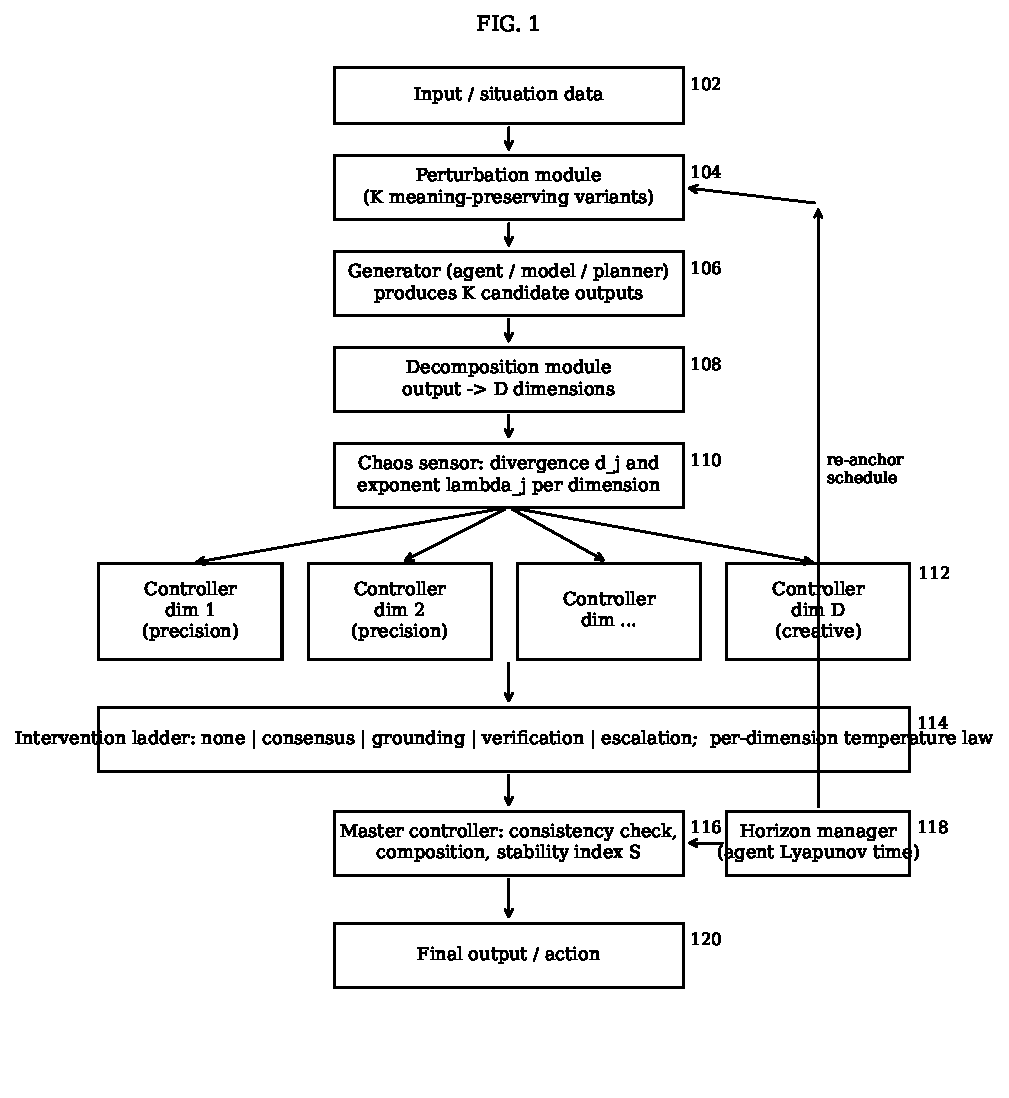
\includegraphics[width=\textwidth,height=0.85\textheight,keepaspectratio]{drawings/fig1_system.pdf}
\end{center}
\newpage
\begin{center}
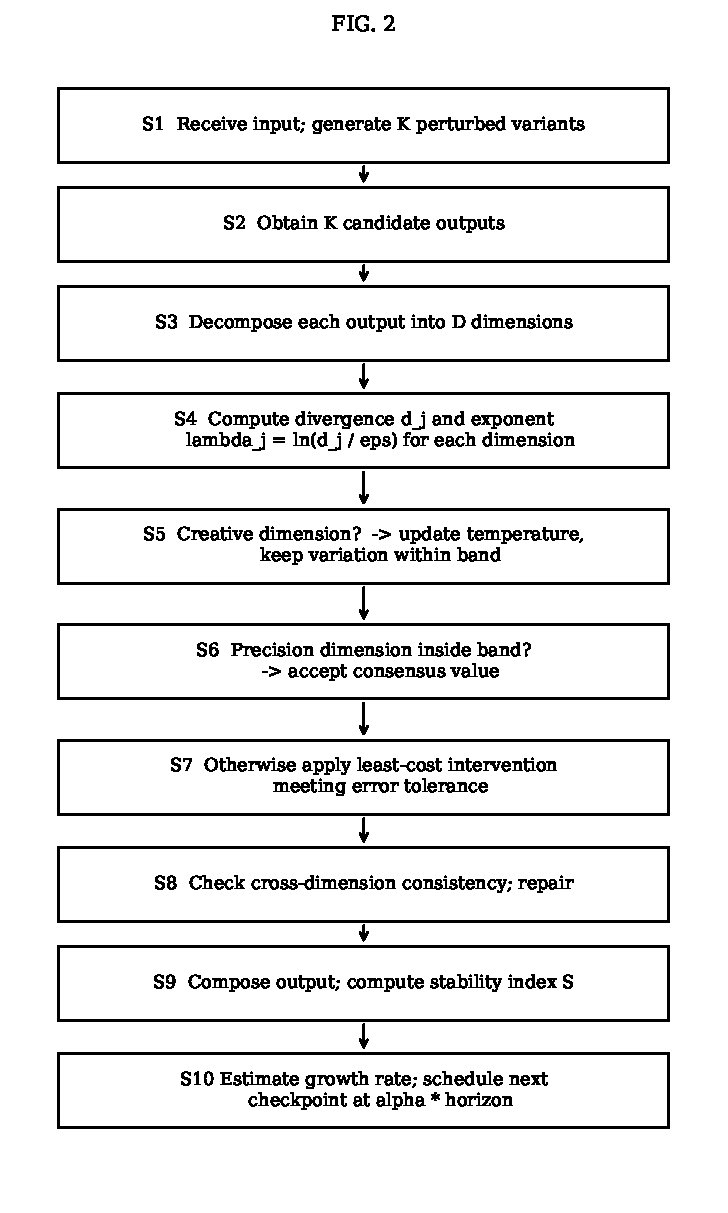
\includegraphics[width=\textwidth,height=0.85\textheight,keepaspectratio]{drawings/fig2_method.pdf}
\end{center}
\newpage
\begin{center}
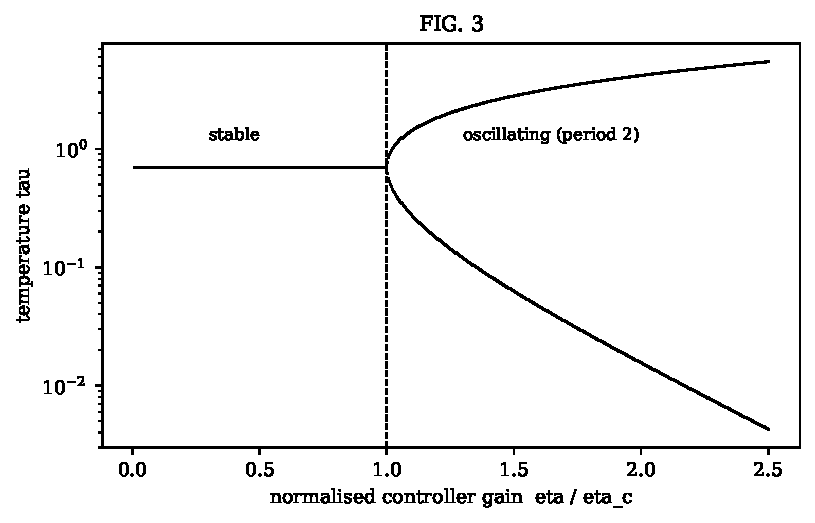
\includegraphics[width=0.85\textwidth]{drawings/fig3_gain_limit.pdf}\\[1cm]
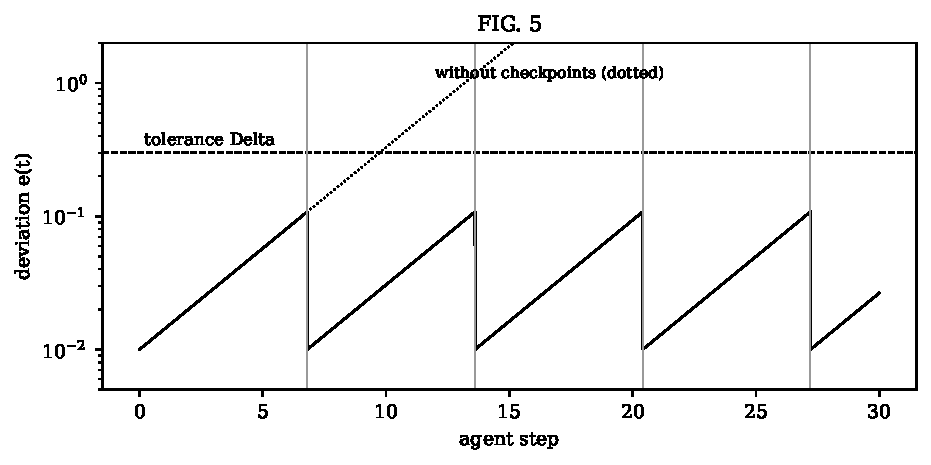
\includegraphics[width=0.85\textwidth]{drawings/fig5_checkpoints.pdf}
\end{center}
\newpage
\begin{center}
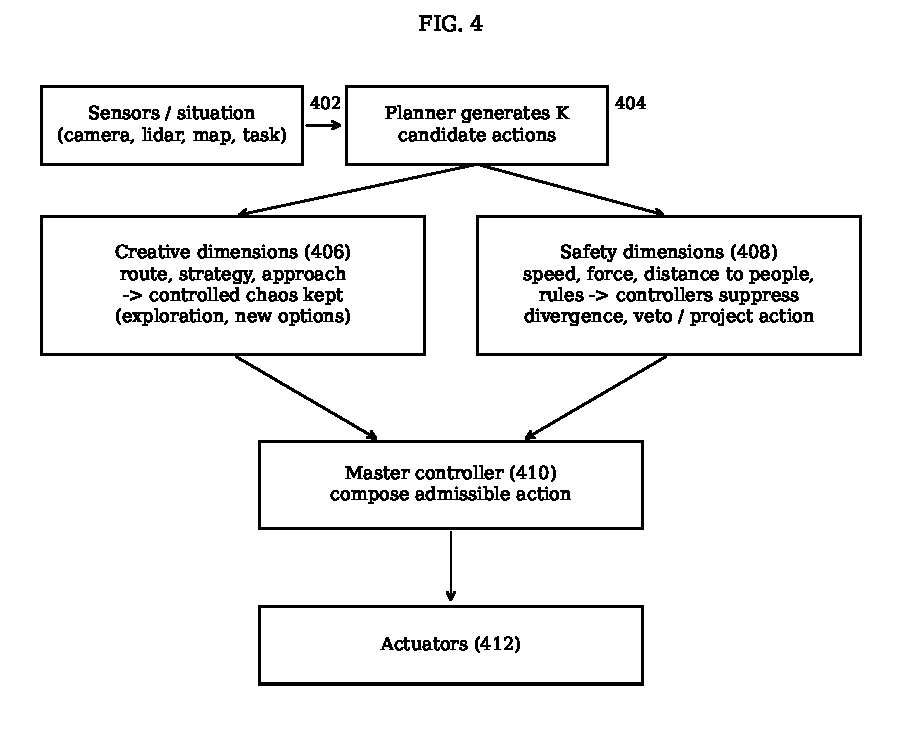
\includegraphics[width=0.95\textwidth]{drawings/fig4_robot.pdf}
\end{center}

\vspace{1cm}
\hfill Signature: \rule{4cm}{0.4pt}\\
\hfill KUHAN K\\
\hfill Applicant

\end{document}
